\chapter[Opis projektu]{Opis projektu}

\section[Treść zadania]{Treść zadania}

\par{Zaprojektować i zaimplementować usługę udostępniania danych statystycznych na temat studentów uczelni wyższej, przy założeniu bezpiecznej i niezawodnej dystrybucji danych wrażliwych - poufnych informacji o studentach.}

\par{Usługa powinna:}
\begin{itemize}


\item mieć dokładnie jeden ten sam tekstowy plik konfiguracyjny dla części 
serwerowej i klientów usługi,
\item składać się po stronie serwerowej z dwóch warstw: (1)  wewnętrznej
  wytwarzającej, przechowującej i przesyłającej przetworzoną wrażliwą
informację, (2) warstwy zewnętrznej do udostępniania przetworzonej informacji
oprogramowaniu klienckiemu usługi,
\item oprogramowanie realizujące część serwerową powinno być współbieżne,
\item składać się po stronie klienckiej z prostych narzędzi opatulających
  zaproponowane API protokołu komunikacyjnego,
\item zapewniać odporność na uszkodzenia węzła, stąd każda z warstw powinna być
  uruchomiona na co najmniej dwóch węzłach,
\item zapewniać realizację usługi w trakcie awarii w czasie obsługi,
\item obsługiwać scenariusz próby ponownego wpięcia się przez węzeł dowolnej z
  warstw, z którym wcześniej utracono łączność, a zarazem być odporną na próbę
zastąpienia nieosiągalnego sieciowo węzła (np. w wyniku ataku DoS, odmowa
usługi) węzłem wrogim do tego nieuprawnionym,
\item na bieżąco i transparentnie dla oprogramowania klienckiego zarządzać
  dostępnymi zasobami lokalizacyjnymi,
\item zapewniać zadany (większy niż 1 ale dopuszczalny konfiguracją mniejszy niż
  liczba serwerów danych) poziom redundancji - z obsługą uzupełniania kopii na
innych serwerach w przypadku awarii włącznie,
\item cała część sewerowa usługi powinna być uruchamiana i zamykana jednokrotnym
  wywołaniem skryptu na jednym węźle serwera z jednym argumentem
<start|stop|status> (wykorzystanie nieinteraktywnych metod automatycznego
uwierzytelniania węzłów w SSH).

\end{itemize}

\section[Wstępny opis rozwiązania]{Wstępny opis rozwiazania}

\par{Nasze rowiązanie to rozproszony system do rejestracji studentów uczelnii wyższych na przemioty. Warstwą wewnątrzną przechowujące dane wrażliwe, w tym przypadku będą węzły rejestrujące studentów ideowo umieszczone w dziekanatach instytutów i obsługiwane przez osoby tam pracujące. Warstwa pośrednia przechowuje informacje o studentach, jednak bez informacji wrażliwej, posiada jedynie dane o istnieniu studenta zapisanego na przedmioty RSO, SOI, ANA1 i SR,  bez imienia, nazwiska i daty urodzenia. Owe informacje są przetwarzane na żądanie aplikacji klienckiej, dostępnej dla studentów, którzy chcą dowiedzieć się, ile osób zapisanych jest na dany przedmiot.}

\section[Wstępny projekt architektury]{Wstępny projekt architektury}

\par{Wewnętrzna warstwa serwera wytwarza i przechowuje informacje na temat studentów uczelni wyższej - stworzone na podstawie danych wprowadzonych przez pracowników dziekanatu. Następnie ów warstwa przesyła informacje do warstwy zewnętrznej serwera (warstwy przetwarzającej) świadczącej usługi udostępniania informacji przetworzonej rozwiązaniom klienckim. Każda z warst komunikować się będzie z użyciem protokołu TCP/IP przesyłając wiadomości zserializowane za pomocą Google Protocols Buffer.}

\begin{figure}[h]
\begin{center}
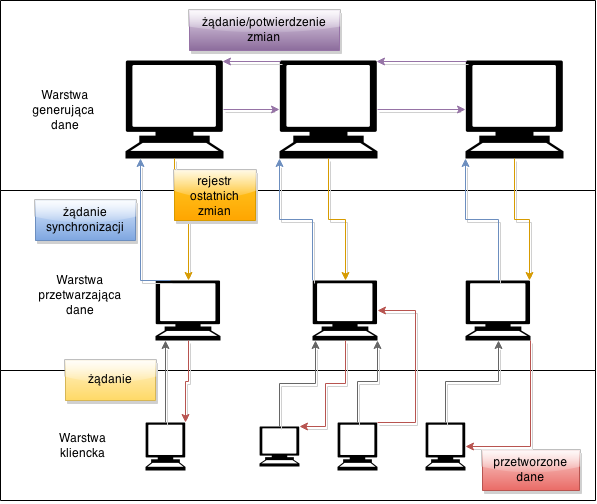
\includegraphics[width=0.9\linewidth]{img/dane_net.png} 
\caption{Diagram ilustrujący komunikację pomiędzy poszczególnymi warstwami}
\label{img:dane_net}
\end{center}
\end{figure}

\subsection*[Warstwa wewnętrzna serwera]{Warstwa wewnętrzna serwera}

\par{Warstwa stworzona w technologii token ring. Węzły połączone są w pierścień i przesyłają sobie kolejno token zawierający informacje o potencjalnych zmianach. Tylko węzeł posiadający token może wykonywać operację aktualizacji danych. Każda zmiana musi być zatwierdzona przez pozostałe węzły. Zapewnia to synchronizację danych oraz bieżące sprawdzenie działania pozostałych węzłów. Szczegółowe informacje na ten temat znajdują się w podrozdziale \ref{z:sw}.}

\par{Dane wrażliwe przechowywane są w postaci rekordów zawierających:}

\begin{itemize}
\item ID studenta
\item imię studenta
\item nazwisko studenta
\item datę urodzenia
\item listę przedmiotów na jakie jest zapisany
\end{itemize}

\par{}

\subsection*[Warstwa zewnętrzna serwera]{Warstwa zewnętrzna serwera (warstwa przetwarzająca)}

\par{Warstwa przeznaczona do komunikacji z aplikacją kliencką. Na żadanie klienta przetwarza wcześniej otrzymane od warstwy wewnętrznej dane i wynik przetwarzania zwraca klientowi. Moduł ten synchronizuje dane okresowo (częstość jest ustalana w pliku konfiguracyjnym), tak aby administrator sam był wstanie dostosować interwał do aktualnych potrzeb. }

\par{Dane o studentach przechowywane są w poniższej postaci:}

\begin{itemize}
\item ID studenta
\item listę przedmiotów na jakie jest zapisany
\end{itemize}

\subsection*[Aplikacja kliencka]{Aplikacja kliencka}

\par{Warstwa przeznaczona dla klienta to z założenia lekka i intuicyjna aplikacja konsolowa. Moduł ten bezpośrednio łączyć będzie się tylko z modułem zewnętrznym serwera. Użytkownik, za pomocą tej aplikacji będzie mógł dowiedzieć się ile osób w danym momencie jest zapisany na wybranie przez niego przedmiot. Aplikacja będzie działała synchronicznie, tzn. po wysłaniu żądania będzie się zawieszała w oczekiwaniu na odpowiedź.}

\section[Opis szczegółowy]{Opis szczegółowy}

\subsection[Założenia]{Założenia}



\subsubsection*[Założenia ogólne]{Założenia ogólne} \label{z:o}

\begin{center}

\begin{tabularx}{\textwidth}{|c|c|X|X|}
\hline
\textbf{ID} & \textbf{Założenie} & \textbf{Szczegóły} & \textbf{Powody decyzji} \\
\hline
\label{z:o1} O1 & 
Protokół TCP/IP & 
Komunikacja między warstwami (wewnętrzna serwera - zewnętrzna serwera jak i zewnętrzna serwera - klienci) odbywa się za pomocą protokołów TCP/IP, wykorzystując Google Protocol Buffer (więcej w podrozdziale \ref{protobuf}).
& Protokół został przez nas wybrany ze względu na elastyczność dla różnych konfiguracji serwerów, tzn. bez względu na to czy warstwy serwera będą działały w obrębie jednego węzła czy nie protokół pozwoli na poprawną komunikację. W przypadku działania obu warstw serwera na jednym komputerze czy nawet w jednym procesie wydajność będzie mniejsza (w porównaniu np. do pamięci współdzielonej), jednak ze względu na ograniczony czas projektu i mniejsze skomplikowanie zostało wybrane to rozwiązanie. \\
\hline

\label{z:o3} O3 & Proste komendy serwera &  
Warstwy serwera będą uruchamiane i zamykane jednokrotnym wywołaniem skryptu na danym węźle serwera z jednym argumentem: start, stop oraz status, które będą kolejno: uruchamiać usługi serwera, wyłączać usługi serwera oraz wyświetlać status serwera. & 
Takie rozwiązanie jest wymagane w treści zadania. Ponadto pozwoli na łatwą obsługę i testowanie części serwerowej systemu. \\
\hline

\end{tabularx}

\subsubsection*[Założenia dotyczące warstwy wewnętrznej serwera]{Założenia dotyczące warstwy wewnętrznej serwera} \label{z:sw}

\begin{tabular}{|c|c|l|l|}
\hline
\textbf{ID} & \textbf{Założenie} & \textbf{Szczegóły} & \textbf{Powody decyzji} \\
\hline
\label{z:sw1} SW1 & Technologia token ring &  Serwery warstwy zewnętrznej połączone są ze sobą w pierścień (każdy ma z góry ustalonego poprzednika i następnika w pliku konfiguracyjnym). Jeśli dany następnik nie odpowiada - brany jest następny adres węzła z listy. W ten sposób bez względu na ilość węzłów mamy zawsze do czynienia z taką samą strukturą (w szczególności - mamy tylko jeden węzeł). Każdy z węzłów wysyła swojemu następnikowi token zawierający informacje odnośnie potencjalnych zmian. & Taka architektura warstwy wewnętrznej pozwala na bieżące sprawdzanie stanu kolejnych węzłów. Jeśli token gdzieś się ,,zagubi'' oznacza to, że dany węzeł uległ awarii. Ponadto taka architektura pozwala na szybką i łatwą synchronizację danych. \\
\hline

\label{z:sw3} SW3 & Bazy danych MySQL & Aplikacja serwerowa wewnętrzna będzie działać w oparciu o relacyjną bazę danych MySQL & 
Baza MySQL jest popularnym systemem relacyjnych baz danych z dobrą dokumentacją oraz szeroką i aktywną społecznością użytkowników. Ponadto system ten jest powszechnie znany wśród wszystkich członków projektu. Dodatkowo MySQL dobrze współpracuje z wybranym językiem programowania Java.
\\
\hline
\label{z:sw4} SW4 & Pełna redundacja danych  &  
Każdy z węzłów wewnętrznych ma pełną i aktualną bazę studentów. Dane są synchronizowane na bieżąco. & 
Natychmiastowa synchronizacja danych i pełna redundancja pozwala uniknąć wielu problemów w trakcie działania serwera, między innymi: dodatkowej synchronizacji po awarii jednego z węzłów, która jest dość problematyczna i skomplikowana. Rozwiązanie to zostało zatwierdzone przez Prowadzącego.\\
\hline
\end{tabular} 

\subsubsection*[Założenia dotyczące warstwy zewnętrznej serwera]{Założenia dotyczące warstwy zewnętrznej serwera} \label{z:sz}

\begin{tabular}{|c|c|l|l|}
\hline
\textbf{ID} & \textbf{Założenie} & \textbf{Szczegóły} & \textbf{Powody decyzji} \\
\hline
\label{z:sz1} SZ1 & Wysyłanie ,,heartbeatów'' &  Węzły zewnętrznej warstwy będą sprawdzały swoją dostępność za pomocą tzw. ,,uderzeń serce'' \textit{(ang. heartbeat)} wysyłanych w danych odstępach czasu (każdy z serwerów musi mieć ustalony ten sam interwał). Dzięki temu będą miały wiedzę na temat aktywności pozostałych serwerów. Brak ,,heartbeata'' od danego serwera po upływie zadanego czasu będzie równoważny z jego brakiem dostępności. & Takie rozwiązanie pozwala na bieżąco monitorować stan poszczególnych węzłów warstwy zewnętrznej. \\
\hline


\end{tabular} 

\subsubsection*[Założenia dotyczące aplikacji klienckiej]{Założenia dotyczące aplikacji klienckiej} \label{z:k}

\begin{tabular}{|c|c|l|l|}
\hline
\textbf{ID} & \textbf{Założenie} & \textbf{Szczegóły} & \textbf{Powody decyzji} \\
\hline
\label{z:k1} K1 & Brak funkcji logowania użytkownika &  
Klient łączy się z systemem identyfikując się jedynie swoim unikatowym ID, które wpisane jest pliku konfiguracyjnym. & 
Decyzja została zatwierdzona przez Prowadzącego. Wynika ona z braku konieczności stworzenia tej funkcjonalności (w związku z minimalnym wpływem na główny cel projektu) oraz na ograniczony czas i mniejszą ilość osób w grupie projektowej niż przewidywana.  \\
\hline
\label{z:k2} K2 & Brak interfejsu graficznego &  Decyzja została zatwierdzona przez Prowadzącego. Wynika ona z braku konieczności stworzenia tej funkcjonalności (w związku z minimalnym wpływem na główny cel projektu) oraz na ograniczony czas i mniejszą ilość osób w grupie projektowej niż przewidywana.  & - \\
\hline

\label{z:k4} K4 & Komunikacja synchroniczna & Aplikacja kliencka będzie się komunikowała z serwerem w sposób synchroniczny. & Ze względu na ograniczoną funkcjonalność aplikacji klienckiej, sprowadzoną jedynie do wysyłania żądań i uzyskiwania odpowiedzi, ten sposób komunikacji wydaje się najbardziej trafny. \\
\hline
\label{z:k5} K5 & Brak funkcji ,,heartbeatu'' & 
Aplikacja kliencka nie będzie na bierząco sprawdzała stanu węzła do którego jest podłączona. Status serwera będzie przez nią sprawdzany jedynie przy logowaniu i wysyłaniu żądania. W przypadku awarii węzła aplikacja będzie przełączała się na kolejny węzeł z listy, aż do skutku. & 
Ze względu na naszą koncepcję aplikacji klieckiej ta funkcjonalność nie jest potrzebna. Z punktu widzenia użytkownika stan serwera interesuje go tylko przy wysyłaniu żądania. System heartbeatów dodaje duży narzut i komplikuje samego klienta nie dając w zamian znacznego wzrostu szybkości działania. W sytuacji awarii i tak musi nastąpić przełączenie na inny węzeł. Różnica polega jedynie na tym, że w przypadku systemu hearbeatów następuje to w momencie upływu określonego czasu bez odpowiedzi serwera, a w przeciwnym - jedynie wtedy kiedy serwer jest potrzebny, tzn. przy logowaniu bądź wysłąniu żądania.\\
\hline
\label{z:k6} K6 & 
Brak interaktywności & Aplikacja kliencka będzie ograniczona jedynie do wywoływania określonych funkcji, według określonego z góry scenariusza. & 
W związku z ograniczonym czasem i głównym celem projektu interaktywna aplikacja kliencka nie jest koniecznością. Funkcjonalność systemu można poprawnie przetestować inicjując konkretne scenariusze (między innymi symulacje awarii czy błędów systemu). Decyzja ta została zatwierdzona przez Prowadzącego.\\
\hline
\end{tabular} 

\end{center}

\subsection[Wymagania funkcjonalne]{Wymagania funkcjonalne}

\begin{tabularx}{\textwidth}{|c|X|X|}
\hline
\textbf{ID} & \textbf{Wymagania}  & \textbf{Powody decyzji} \\
\hline

\label{z:WF1} WF1 & \textbf{Plik konfiguracyjny}


 Każdy z węzłów danej warstwy będzie posiadała plik konfiguracyjny o tej samej strukturze. W zależności od typu dane z pliku zostaną odpowiednio skonfigurowane. Plik będzie zawierał: ID węzła, listę serwerów (zależnie od typu - zewnętrznych lub wewnętrznych), dodatkowe dane konfiguracyjne (np. odpowiadających za redundancję danych, okresową synchronizację, itd.) &
Takie rozwiązanie jest wymagane w treści zadania. Ponadto ujednolica i ułatwia konfigurację projektu bez potrzeby ponownej kompilacji.\\
\hline

\label{z:WF2} WF2 &  \textbf{Zmiana jednego rekordu na raz }

Jeśli dany węzeł chce dodać/usunąć/zmodyfikować dane o studencie musi posiadać token, który przesyła do kolejnych serwerów na końcu otrzymując potwierdzenie, że każdy z węzłów wprowadził żądaną zmianę. & 
Ze względu na to, że w sieci warstwy wewnętrznej serwera istnieje jeden token jest sensowne przyjąć założenie, że na raz można wprowadzić jedną modyfikację w bazie. Ponadto pozwala to utrzymać nieduży rozmiar tokena, co sprzyja jego szybszemu przesyłaniu między węzłami. Nawet w przypadku wielu żądań (od każdego węzła jedno) powinno to działać na tyle szybko, że osoby wprowadzające dane nie odczują opóźnienia. Dodatkowo wprowadzanie pojedynczych informacji pozwala na szybsze wykrycie awarii węzła serwera oraz zaoszczędza większej ilości czasu, niż w przypadku wpisywania dużej ilości danych na raz, a dopiero potem sprawdzania czy węzeł działa poprawnie. \\
\hline

\end{tabularx}
\newpage
\begin{tabularx}{\textwidth}{|c|X|X|}
\hline
\textbf{ID} & \textbf{Wymagania}  & \textbf{Powody decyzji} \\
\hline

\label{z:WF3} WF3 & \textbf{Okresowa synchronizacja }

 Synchronizacja z warstwą wewnętrzną następuje okresowo, w danych odstępach czasu, sterowanych za pomocą pliku konfiguracyjnego. Jest ona wykonywana na rządanie węzłów warstwy zewnętrznej. Synchronizacja polega na pobraniu jedynie zmienionych rekordów bazy, a nie wszystkich. Ostatnia funkcjonalność zostanie rozwiązana za pomocą, tzw. ,,znaczników czasu'' \textit{(ang. timestamp)}. & Synchronizacja o konkretnych porach pozwala na odpowiednie rozporządzanie pracą systemu. W przypadku rzadkiej modyfikacji danych przez warstwę wewnętrzną serwera synchronizacja może być wykonywana, np. raz na dzień. Z drugiej strony można ustawić synchronizację co 1 sekundę, co spowoduje wrażenie ciągłej synchronizacji (oczywiście nie biorąc pod uwagę potencjalnych opóźnień). Takie rozwiązanie pozwala administratorowi na odpowiednią optymalizację działania systemu. Dzięki aktualizacji jedynie konkretnych danych, a nie bazy w całości jest to stosunkowo szybkie. \\
\hline

\label{z:WF4} WF4 & \textbf{Redundacja danych }

W zależności od zmiennej ustawionej w pliku konfiguracyjnym warstwa przetwarzająca może posiadać pełną redundancję bądź nie. Przyjmuje się, że minimalna liczba serwerów posiadających w pełni aktualne dane to 3. & To założenie służy spełnieniu warunków zadania. Możliwość modyfikacji poziomu redundancji pozwala dopasować system do ilości węzłów w warstwie zewnętrznej serwera i do danego zapotrzebowania.\\
\hline

\label{z:WF5} WF5 & \textbf{Udostępnianie usług }

 Warstwa zewnętrzna obsługuje żądania klientów realizując usługę zwracania ilości studentów zapisanych na dany przedmiot. Serwer nasłuchuje czekając na żądania, a następnie (w ramach możliwości) je spełnia. & To założenie służy spełnieniu warunków zadania. \\
\hline



\label{z:WF6} WF6 & \textbf{Obliczanie danych statystycznych }

  Serwery zewnętrzne, zwane też przetwarzającymi, otrzymują dane od warstwy wewnętrznej, jednak zapisują z nich jedynie dane niewrażliwe używając ich do wyliczania ilości studentów zapisanych na dany przedmiot. Do tej operacji pełne informacje o studentach nie są potrzebne. & 
To założenie służy spełnieniu warunków zadania. \\
\hline

\end{tabularx}
\newpage
\begin{tabularx}{\textwidth}{|c|X|X|}
\hline
\textbf{ID} & \textbf{Wymagania}  & \textbf{Powody decyzji} \\
\hline

\label{z:WF7} WF7 & \textbf{Dostęp do usługi pobrania danych statystycznych} 
 
Aplikacja kliencka po połączeniu z serwerem zewnętrznym może pobrać informacje na temat ilości studentów zapisanych na dany przedmiot. Użytkownik otrzymuje jedynie nazwę przedmiotu i liczbę zapisanych studentó, bez dostępu do danych wrażliwych. Może być wysyłane jedno żądanie na raz od danego użytkownika. Nie ma funkcji agregacji wielu żądań w jedno. & 
Jest to dobry przykład funkcjonalności, która zabezpiecza nam dane wrażliwe przed zwyczajnym użytkownikiem, udostępniając jedynie informacje, które mogą być publiczne. Agregacja bądź wysyłanie wielu żądań na raz nie jest konieczne do sprawdzenia poprawnego działania systemu i nie zmienia w żaden sposób wizji funkcjonowania systemu.\\
\hline



\end{tabularx}

\subsection[Wymagania niefunkcjonalne]{Wymagania niefunkcjonalne}

\section[Potencjalne problemy]{Potencjalne problemy}

\subsection*[Podłączenie nowego serwera warstwy wewnętrznej]{Podłączenie nowego serwera warstwy wewnętrznej}

\subsection*[Podłączenie nowego serwera warstwy zewnętrznej]{Podłączenie nowego serwera warstwy zewnętrznej}

\subsection*[Awaria węzła warstwy wewnętrznej]{Awaria jednego z węzłów warstwy wewnętrznej}

\par{W przypadku awarii wewnętrznego węzła serwera musimy rozważyć kilka scenariuszy:}

\begin{itemize}

\item \textbf{Brak tokena, brak oczekującej operacji} - 

\item \textbf{Brak tokena, oczekująca operacja} - 

\item \textbf{Posiada token, brak oczekujących operacji} - 

\item \textbf{Posiada token, oczekująca operacja} - 

\end{itemize}

\subsection*[Awaria węzła warstwy zewnętrznej]{Awaria jednego z węzłów warstwy zewnętrznej}

\subsection*[Kwestia równomiernego podziału klientów między serwery oraz serwerów zewnętrznych między wewnętrzne]{Kwestia równomiernego podziału klientów między serwery oraz serwerów zewnętrznych między wewnętrzne}

\subsection*[Kwestia rozmieszczenia warstw serwera w obrębie jednego komputera bądź wielu odrębnych]{Kwestia rozmieszczenia warstw serwera w obrębie jednego komputera bądź wielu odrębnych}


\section[Organizacja środowiska programistycznego]{Organizacja środowiska programistycznego}